\chapter{Diseño e implementación} % Main chapter title

\label{Chapter3} % Change X to a consecutive number; for referencing this chapter elsewhere, use \ref{ChapterX}

\definecolor{mygreen}{rgb}{0,0.6,0}
\definecolor{mygray}{rgb}{0.5,0.5,0.5}
\definecolor{mymauve}{rgb}{0.58,0,0.82}

%%%%%%%%%%%%%%%%%%%%%%%%%%%%%%%%%%%%%%%%%%%%%%%%%%%%%%%%%%%%%%%%%%%%%%%%%%%%%
% parámetros para configurar el formato del código en los entornos lstlisting
%%%%%%%%%%%%%%%%%%%%%%%%%%%%%%%%%%%%%%%%%%%%%%%%%%%%%%%%%%%%%%%%%%%%%%%%%%%%%
\lstset{ %
  backgroundcolor=\color{white},   % choose the background color; you must add \usepackage{color} or \usepackage{xcolor}
  basicstyle=\footnotesize,        % the size of the fonts that are used for the code
  breakatwhitespace=false,         % sets if automatic breaks should only happen at whitespace
  breaklines=true,                 % sets automatic line breaking
  captionpos=b,                    % sets the caption-position to bottom
  commentstyle=\color{mygreen},    % comment style
  deletekeywords={...},            % if you want to delete keywords from the given language
  %escapeinside={\%*}{*)},          % if you want to add LaTeX within your code
  %extendedchars=true,              % lets you use non-ASCII characters; for 8-bits encodings only, does not work with UTF-8
  %frame=single,	                % adds a frame around the code
  keepspaces=true,                 % keeps spaces in text, useful for keeping indentation of code (possibly needs columns=flexible)
  keywordstyle=\color{blue},       % keyword style
  language=[ANSI]C,                % the language of the code
  %otherkeywords={*,...},           % if you want to add more keywords to the set
  numbers=left,                    % where to put the line-numbers; possible values are (none, left, right)
  numbersep=5pt,                   % how far the line-numbers are from the code
  numberstyle=\tiny\color{mygray}, % the style that is used for the line-numbers
  rulecolor=\color{black},         % if not set, the frame-color may be changed on line-breaks within not-black text (e.g. comments (green here))
  showspaces=false,                % show spaces everywhere adding particular underscores; it overrides 'showstringspaces'
  showstringspaces=false,          % underline spaces within strings only
  showtabs=false,                  % show tabs within strings adding particular underscores
  stepnumber=1,                    % the step between two line-numbers. If it's 1, each line will be numbered
  stringstyle=\color{mymauve},     % string literal style
  tabsize=2,	                   % sets default tabsize to 2 spaces
  title=\lstname,                  % show the filename of files included with \lstinputlisting; also try caption instead of title
  morecomment=[s]{/*}{*/}
}


En este capítulo se describe cómo se han utilizado las herramientas mencionadas en el capítulo \ref{Chapter2} y sus integraciones. Se presenta la arquitectura de alto nivel completa y luego se describe parte por parte desde el consumo de datos hasta la salida del proceso y su almacenamiento.


\section{Arquitectura del sistema}

En la figura \ref{fig:arqsistema} se puede observar la arquitectura de alto nivel que integra las herramientas utilizadas en la fase de entrenamiento y evaluación de los modelos de IA con las herramientas utilizadas para el despliegue.

\begin{figure}[htbp]
	\centering
	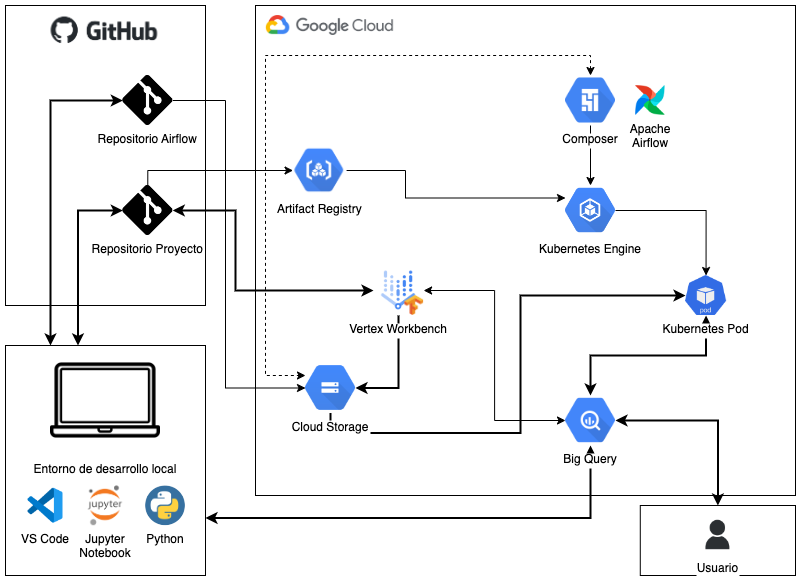
\includegraphics[width=1\textwidth]{./Figures/arq-sistema.png}
	\caption{Diagrama de la arquitectura de alto nivel.}
	\label{fig:arqsistema}
\end{figure}

La mayor parte del desarrollo se realizó en una computadora local, que contaba con un intérprete de Python y Visual Studio Code con Jupyter para la escritura de código. Estos archivos se sincronizaban contra un repositorio de GitHub.

Los datos para realizar el entrenamiento de los modelos de IA fueron tomados del \textit{data warehouse} BigQuery utilizando consultas SQL y bibliotecas de Google para Python para manejar su ejecución.

Estos datos son llevados a BigQuery por un proceso ajeno a este desarrollo, que se encarga de sincronizar la base de Salesforce hacia el \textit{data warehouse} diariamente. Particularmente, hay una tabla que contiene los reclamos y consultas de los usuarios, con su identificador de caso, fecha de creación y estado.

En las ocasiones que las que fue necesario un mayor poder de cómputo a través del uso de una placa de vídeo dedicada, se utilizó una instancia de Vertex AI Workbench en la nube de Google. Por lo general, estas situaciones se dieron al momento de realizar distintas pruebas con las redes neuronales BERT. Los modelos eran luego exportados al almacenamiento de la nube llamado Cloud Storage en formato ``Pickle'' o ``HDF5'' \textit{(Hierarchical Data Format 5)}.

El repositorio del proyecto cuenta con un Workflow de GitHub Action que se corre manualmente y genera una imagen de Docker, incluyendo bibliotecas y librerías necesarias, archivos de código y de configuración. Esta imagen de Docker es enviada al Artifact Registry de la nube de Google y almacenada allí.

Por otro lado, se trabajó en otro repositorio separado, que es único para manejar todos los flujos de trabajo de Apache Airflow que tiene el área de \textit{machine learning}. Este repositorio es exclusivo para la etapa de despliegue, y se agregó el DAG que administra el proceso de predicción.

El repositorio de Airflow cuenta con un Workflow de GitHub Action que sincroniza el código de los DAGs contra un Cloud Storage que está conectado a la instancia del orquestador. Airflow periódicamente controla si hay un flujo de trabajo nuevo y cuando lo detecta, lo carga.

Al momento de ejecutar el proceso, Airflow utiliza un operador dentro del DAG para conectarse con la plataforma de Kubernetes en instancia un Pod. Este Pod ejecuta los archivos de código del contenedor que se empaquetaron en la imagen de Docker cargada previamente en el Artifact Registry.

Al finalizar, se guardan los resultados de las predicciones en una tabla en BigQuery y el Pod es eliminado de Kubernetes. Los datos quedan disponibilizados en la base para que cualquier usuario con los suficientes permisos pueda consumirlos ejecutando una consulta a la base.

\section{Extracción y preprocesamiento del texto}


\section{Entrenamiento de los modelos}


\section{Desarrollo de GitHub Actions}


\section{Empaquetamiento del código y artefactos}


\section{Desarrollo del \textit{pipeline} de predicción}


\section{Almacenamiento de predicciones}

